%!Tex Root = ../main.tex
% ./Packete.tex
% ./Design.tex
% ./Deklarationen.tex
% ./Vorbereitung.tex
% ./Aufgabe1.tex
% ./Aufgabe2.tex
% ./Aufgabe4.tex
% ./Appendix.tex

\section{Aufgabe 3}

\setcounter{exercise}{1}

\begin{frame}[allowframebreaks]{Aufgabe \thesection}{Programmable Logic Arrays}
  
        \begin{requirementsnoinc}
            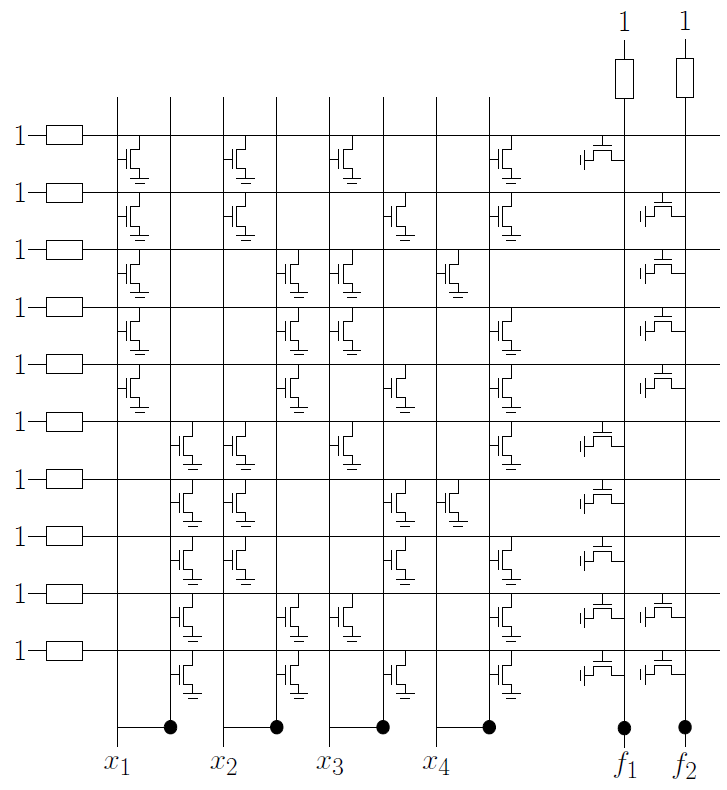
\includegraphics[height=0.4\textwidth, center]{figures/PLA.png}
        \end{requirementsnoinc}

        \begin{exercisenoinc}
            Gesucht sind die beiden Polynome $f_1,f_2 \in \mathbb{B}_4$, die durch dieses PLA implementiert werden
        \end{exercisenoinc}
        \begin{solution}
            $f_1 = \bar x_1 \bar x_2 \bar x_3 x_4 + x_1 \bar x_2 \bar x_3 x_4 + x_1 \bar x_2 x_3 \bar x_4 +  x_1 \bar x_2 x_3 x_4 +  x_1 x_2 \bar x_3 x_4 +  x_1 x_2 x_3 x_4$ \newline
            $f_2 = \bar x_1 \bar x_2  x_3 x_4 + \bar x_1 x_2 \bar x_3 \bar x_4 + \bar x_1 x_2 \bar x_3 x_4 +  \bar x_1 x_2 x_3 x_4 +  x_1 x_2 \bar x_3 x_4 +  x_1 x_2 x_3 x_4$
        \end{solution}

        \begin{exercisenoinc}
            Kosten des PLA
        \end{exercisenoinc}
        \begin{solution}
            Primäre Kosten $cost_1(f_1, f_2) = 10$ (Zeilen des PLA bzw. Anzahl der Monome) \\
            Sekundäre Kosten $cost_2(f_1, f_2) = 52$ (Zahl der Transistoren im PLA)
        \end{solution}

        \begin{exercisenoinc}
            Hypercubes von $f_1$ und $f_2$ zeichnen
        \end{exercisenoinc}

        \begin{solutionnoinc}
          \begin{figure}
            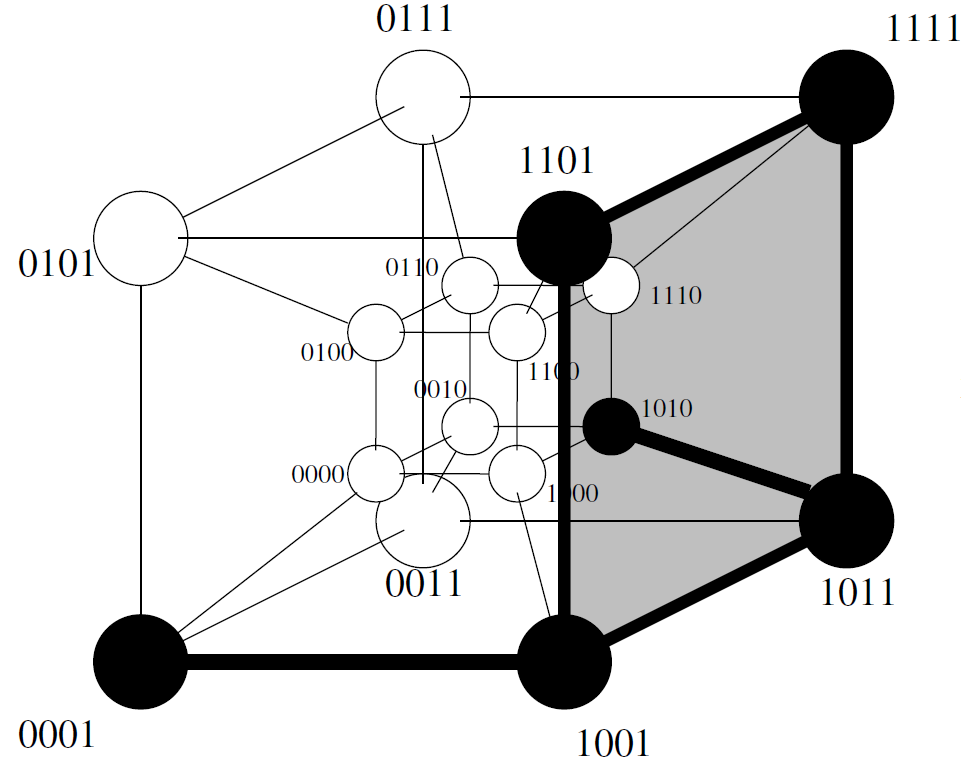
\includegraphics[scale=0.2, center]{figures/Hypercubef1.png}
            \caption{Funktion $f_1$}
          \end{figure}
        \end{solutionnoinc}

        \begin{solution}
          \begin{figure}
            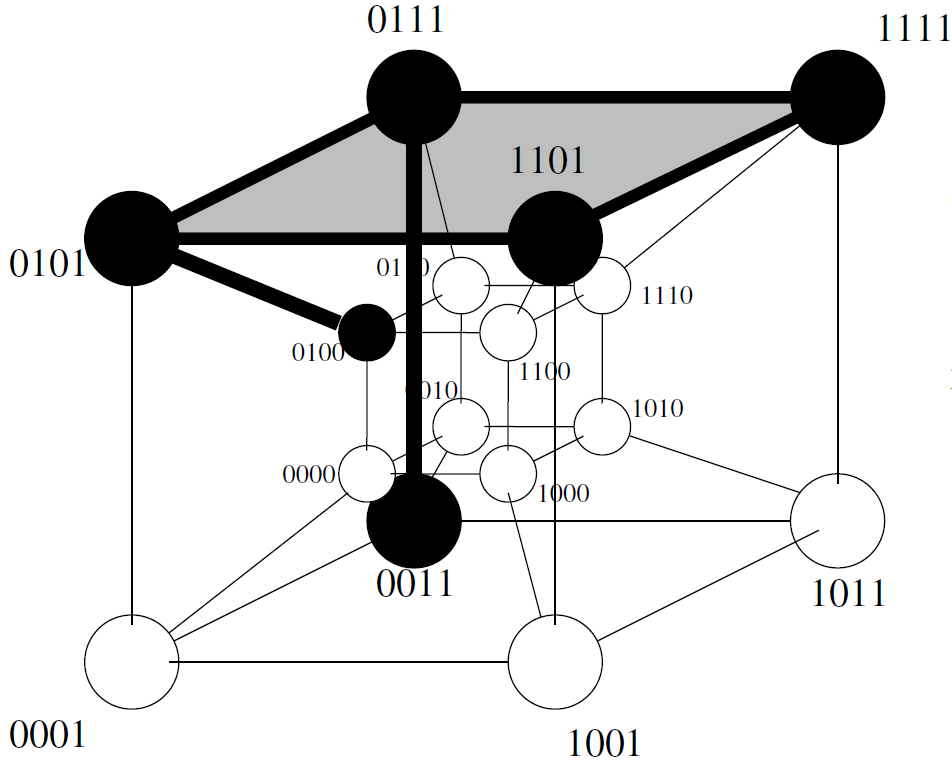
\includegraphics[scale=0.2, center]{figures/Hypercubef2.png}
            \caption{Funktion $f_2$}
          \end{figure}
        \end{solution}
    \end{frame}
